\chapter{Methodologies}
This chapter is about the material and research methods that will be used for this project. The methodologies are important in research to help with the design and evaluation of the project. 
\section{Design Science}
“Design science research is a method that establishes and operationalizes research when the desired goal is an artefact or a recommendation” \cite{Dresch}. It includes users, the developers and research experts of various backgrounds.
Figure \ref{fig:Hevner2007} refers to the environment in which the artefact is observed, the environment is the people, the organizations and the technology. Design science research supports the development of the artefact that solves a problem and the goal is to increase the existing knowledge base. The artefact is evaluated and justified and the knowledge base can be used for the existing foundations and methods that are recognized by the scientific community.

The relevance cycle goes from requirements and field testing to the design cycle and rigor cycle and then adds to the knowledge base.
\begin{figure}[H]
    \centering
    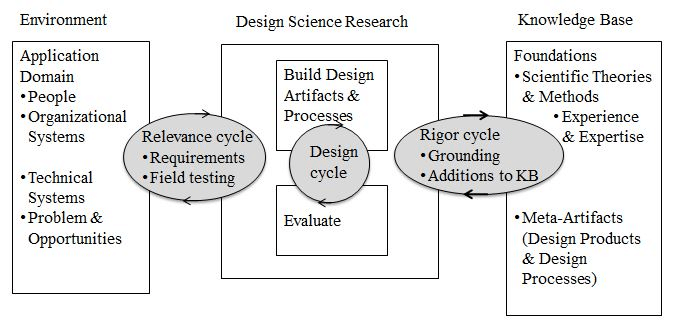
\includegraphics[width=120mm]{figures/Design-Science-Research-Cycles-Hevner-2007.png}
    \caption{Design science in information science research \cite{Hevner2007}}
    \label{fig:Hevner2007}
\end{figure}

Hevner et al \cite{Hevner2004} lists seven criteria that are essential for design research. The first criteria is the creation of a new artefact that has to solve a specific problem. The utility of the artefact has to be explained and later evaluated. The contribution of the artefact has to be clarified for academics and professionals interested in solving problems to increase the knowledge of the area. The validity of the artefact has to be rigorously tested and demonstrated to show that the artefact is suitable for the proposed use. The researchers have to understand the problem, and the results should be communicated in a proper way to those that are interested in the area.

Hevner and Chatterjee suggests a checklist for researchers to ensure that all the key aspects of design science research are being covered \cite{Hevner2010}. The questions from the checklist can be seen on page \pageref{tab:1} . Design science includes the users, developers and experts with a variety of backgrounds. With documentation about the research process it is possible to get a good development process with relevant results to the research.

\newpage
\begin{table}[H]
\begin{tabular}{ |l|l| }
  \hline
  \multicolumn{2}{|c|}{Questions} \\
  \hline
1 & What is the research question (design requirements)?\\ 
\hline
2 & What is the artifact? How is the artifact represented?\\
\hline
3 & What design processes (search heuristics) will be used to build the artifact?\\ 
\hline
4 &\makecell[l]{ How are the artifact and the design processes grounded by the knowledge base? \\What, if any, theories support the artifact design and the design process?} \\
\hline
5 &\makecell[l]{ Which evaluations are performed during the internal design cycles?\\ Which design improvements are identified during each design cycle?}\\ 
\hline
6 & \makecell[l]{How is the artifact introduced into the application environment and how is it field tested?\\ What metrics are used to demonstrate artifact utility and improvement over previous artifacts?}\\ 
\hline
7 &\makecell[l]{ What new knowledge is added to the knowledge base and in what form \\ (e.g., peer-reviewed literature, meta-artifacts, new theory, new method)?}\\ 
\hline
8 & Has the research question been satisfactorily addressed?\\
 \hline
  
\end{tabular}
\label{tab:1}
\caption{A checklist for researchers, key aspects of design science research}
\end{table}

\section{Conceptual Design} \label{concept}
Conceptual design uses the established requirements for the application and transforms it into a conceptual model\cite{interactiondesignbook}, the model shows the main functionalities of the application and lets the users interact with it. The key principles of conceptual design is to have an open mind, but not forget the users and their context. To discuss the ideas with other stakeholders. Use prototyping to get rapid feedback and do many iterations \cite{interactiondesignbook}. A conceptual model is very beneficial in the beginning phase of development.
\section{Prototyping} \label{interactiondesign}
Prototypes are a simplified version of an artefact design that are created with the purpose to test design features. “Prototyping is a key activity within the design of interactive systems” \cite{Buchenau}. Users are able to test and evaluate functionalities of the system before the artefact is finished and give feedback.  The evaluation and feedback from the prototype testing will lead to improvements of the prototype. Prototypes are divided between levels of fidelity, ranging from low-fidelity to high-fidelity. This research project will use three different levels of fidelity for the prototyping.

Low-fidelity prototyping \cite{interactiondesignbook} can be used to create a layout and test different design options. Low-fidelity prototyping includes three different methods that will be used in to project.

1. Sketching, cheap and time effective way of testing different design options, drawn by hand.

2. Wireframing, represents the layout and the content.

3. Mock-up, displays how the design looks with colours, content and in-depth descriptions.

Mid-fidelity prototyping is a mixture between the correct content and some functionality.

High-fidelity prototyping is closer to the end product of the application. With this prototype it is easier to do usability evaluation and let users test the functionalities and look at the content-

\section{Design Principles}
Design principles \cite{DesignP} are guidelines and design considerations which interaction designers focuses on for the user experience and user interface of a product. There are five principles that are important to consider while integrating features for an interface.

Visibility is the first principle that states that the more visible an item is, the more likely a user will know it and use it. \cite{Norman} The user interface should be intuitive.

Feedback is the principle of making it clear what action has been taken and what has been accomplished \cite{Norman}. The user should not have to guess what their action accomplished and there should be feedback in the form of visual, tactile or audio.

Constraints is about limiting the range of interaction possibilities for the user to simplify the interface and guide the user to the appropriate next action \cite{Norman}. Constraints makes it harder for a user to make mistakes.

Consistency refers to having similar operations and similar elements for achieving similar tasks \cite{Norman}. The design should not have any surprises.

Affordance refers to an attribute of an object that allows people to know how to use it \cite{Norman}, by using symbols that users are accustomed to, they will already understand what the action is. 


\section{Data Gathering}
This chapter covers the evaluation methods that will be used for this project. The evaluation methods are important for the research rigor and design research process to demonstrate the utility, quality and efficacy of the artefact.
Quantitative methods are focused on gathering large quantities of data and is collected through polls, questionnaires, surveys and more. The data can be used for statistical analysis.
The qualitative research in this project will be based on semi-structured interviews, observations and focus groups. Qualitative research focuses more on in-depth research and fewer data collection cases.

\subsection{Literature Review}
A literature review is gathering of published articles, reports, books and other relevant documents by searching with keywords in academic journals and search engines. The literature review shows a summary of relevant information about methods, data gathering and what the research accomplished. The literature review can contribute to finding and establishing requirements for the artefact development.

\subsection{Semi-Structured Interview}
Semi-structured interviews uses pre-defined questions to create a structure of an interview. The prepared questions are asked and are open for answers and discussions. The method allows for follow up questions and exploring discussions. This method was used during the interviews with ... An interview guide approved by NSD can be found in appendix ..

\subsection{Survey}
A survey is a quantitative method of gathering data with the purpose to produce statistics about some aspects of a sample population. A survey collects information by asking people questions and the answers are the data that is analyzed \cite{fowler2013survey}. The questions are mainly close-ended with few open-ended questions at the end for free form answers.
\subsection{Focus Groups}
A focus group is a group interview with several participants at the same time with a moderator present to ask questions and guide the conversation. “Focus groups explicitly use group interaction as part of the method. This means that instead of the researcher asking each person to respond to a question in turn, people are encouraged to talk to one another: asking questions, exchanging anecdotes and commenting on each other's experiences and points of view”\cite{Kitzinger}. The experiences and points of view can be used to identify common knowledge and get feedback in a setting that is more relaxed than in a laboratory. The focus group will consist of many members. 

\subsection{Case Study}
A case study is an intensive study about a person, a group of people or a unit where the aim is to generalize over several units \cite{Heale7}. In this project, a group of people were asked to explain how they log their workouts and how they would interact with the application.
\section{Evaluation of Prototypes}
Evaluating a prototype is part of the developmental phase and is performed at the end of each iteration. There are different ways of evaluating a prototype. Experts and users can be included to be certain that the prototype is relevant and the design is easy to use, easy to learn and the design is intuitive. 

\subsection{Usability Testing}
Usability testing is testing a prototype with participants that represent real users \cite{dumas1999practical} . The users play around with the prototype and perform real tasks while their actions are observed and notes are taken. The goal of a usability test is to improve the usability of a product, analyse data and find problems and reiterate the development phase to improve the prototype.
\subsection{System Usability Scale}
Another way of evaluating HCI is to use the system usability scale by John Brooke \cite{Brooke}. This evaluation method differs from the heuristic evaluation by having regular users that are not experts in the field of HCI to evaluate the system. The system usability scale consists of ten statements, every statement gets a score where strongly disagree is the weakest and strongly agree is the strongest.
The SUS score can be calculated and there are different ways of measuring it, grades, adjectives or percentages can be used \cite{doi:10.1080/10447318.2018.1455307} . The ten statements are structured so that odd numbers have positive loaded questions and even numbers have negative loaded questions. To calculate the score, the odd numbers will have 1 subtracted from their value and the even numbers will subtract their number from the value 5. Adding this together and then multiplying it with 2.5 will get a SUS score out of 100. A SUS score above 68 is considered as a good score \cite{doi:10.1080/10447318.2018.1455307}. 
\begin{figure}[H]
    \centering
    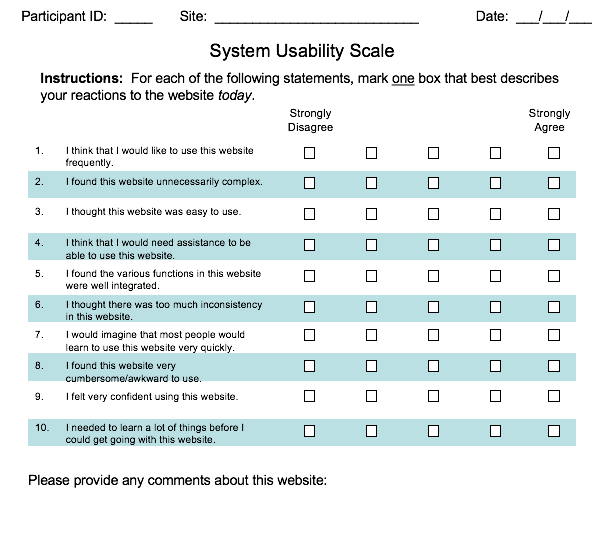
\includegraphics[width=120mm]{figures/sus-template.png}
    \caption{System usability scale template}
\end{figure}


\subsection{Nielsen`s Heuristics} \label{nielsen}
To evaluate the usability of a system, Nielsen \cite{Nngroup} developed ten heuristics as a guideline to test and estimate the usability of a product. The ten heuristics can be used by human computer interaction experts to evaluate the interface of an application. The evaluation is performed by a small set of usability experts individually and only requires a few experts to identify 75\% of the problems \ref{NN}.

\begin{figure}[H]
    \centering
    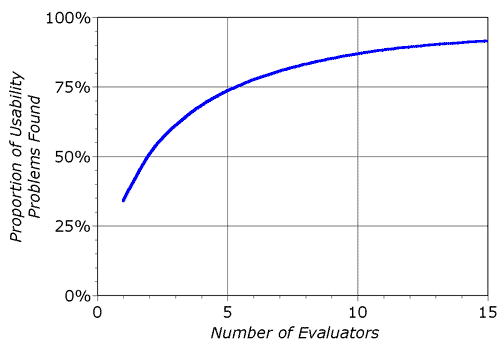
\includegraphics[width=120mm,height=8cm,keepaspectratio]{figures/heur_eval_finding_curve.png}
    \caption{The proportion of usability problems in an interface using various numbers of evaluators\cite{Nngroup}}
    \label{NN}
\end{figure}
Nielsen`s heuristics will be tested by experts in information science.

\begin{table}[H]
\hskip-1.5cm\begin{tabular}{ |l|l| }
  \hline
  \multicolumn{2}{|c|}{Nielsen`s Heuristics} \\
  \hline
\makecell[l]{Visibility of system\\ status} &\makecell[l]{The system should always keep users informed about what is going on,\\ through appropriate feedback within a reasonable time.}\\ 
\hline
\makecell[l]{Match between the\\ system and the real world} &\makecell[l]{ The system should speak the users' language, with words, phrases, and\\ concepts familiar to the user, rather than system-oriented terms. Follow\\ real-world conventions, making information appear in a natural and\\ logical order.}\\
\hline
\makecell[l]{User control and\\ freedom} & \makecell[l]{Users often choose system functions by mistake and will need a clearly\\ marked "emergency exit" to leave the unwanted state without having to\\ go through an extended dialogue. Support undo and redo.}\\ 
\hline
\makecell[l]{Consistency and\\standards}  & \makecell[l]{Users should not have to wonder whether different words, situations,\\ or actions mean the same thing. Follow platform conventions.} \\
\hline
\makecell[l]{Error prevention} & \makecell[l]{Even better than good error messages are a careful design which prevents\\ a problem from occurring in the first place. Either eliminate error-prone\\ conditions or check for them and present users with a confirmation option\\ before they commit to the action.}\\ 
\hline
\makecell[l]{Recognition rather than\\ recall} & \makecell[l]{Minimize the user's memory load by making objects, actions, and options\\ visible. The user should not have to remember information from one part\\ of the dialogue to another. Instructions for use of the system should be\\ visible or easily retrievable whenever appropriate.}\\ 
\hline
\makecell[l]{Flexibility and\\ efficiency of use} & \makecell[l]{Accelerators — unseen by the novice user — may often speed up the\\ interaction for the expert user such that the system can cater to both\\ inexperienced and experienced users. Allow users to tailor \\frequent actions.}\\ 
\hline
\makecell[l]{Aesthetic and\\ minimalist design} & \makecell[l]{Dialogues should not contain information which is irrelevant or rarely\\ needed. Every extra unit of information in a dialogue competes with\\ the relevant units of information and diminishes their relative visibility.}\\
\hline
\makecell[l]{Help users recognize,\\ diagnose, and recover\\ from errors} &\makecell[l]{Error messages should be expressed in plain language (no codes),\\ precisely indicate the problem, and constructively suggest a solution.}\\
\hline
\makecell[l]{Help and documentation}&\makecell[l]{Even though it is better if the system can be used without documentation,\\ it may be necessary to provide help and documentation. Any such\\ information should be easy to search, focused on the user's task,\\ list concrete steps to be carried out, and not be too large.}\\
  \hline
  
\end{tabular}
\label{tab:2}
\caption{Nielsen`s heuristics to follow for user interface}
\end{table}



\newpage

\subsection{Obervations}
Another qualitative method to evaluate an application is observations. “Individuals are observed performing specified tasks within a controlled environment”\cite{Preece}. The evaluator has a script and predetermined tasks for the participants. They are encouraged to communicate while they are performing the tasks and use the think-aloud technique which is a technique developed by Erickson and Simon\cite{Erickson2}. The technique requires the participants to say out loud what they are thinking and trying to do. Thus making it easier for the evaluator to take notes, which can be analyzed later.

